\chapter{Conservação da massa e equações balanceadas}\label{ch:g8:balanced-equations}

Uma tora de dois quilogramas \omterm{def:g4:what-a-fire-needs:burning}{queima} numa lareira. De manhã, sobram
algumas dezenas de gramas de cinza cinzenta. Será que quase dois
quilogramas de matéria desapareceram durante a noite? Durante séculos,
ninguém soube responder. A resposta veio de um químico que decidiu pesar
tudo --- inclusive os gases, que ninguém tinha pensado em pesar.

\begin{recall}
Numa \omterm{def:g7:chemical-reactions:reaction}{reação química}, os \omterm{def:g7:chemical-reactions:reactant}{reagentes} são consumidos e os produtos são
formados; os \omterm{def:g7:atoms-and-molecules:atom}{átomos} dos \omterm{def:g7:chemical-reactions:reactant}{reagentes} se rearranjam nos produtos, sem serem
criados nem destruídos (\cref{ch:g7:chemical-reactions}). Uma \omterm{def:g7:atoms-and-molecules:formula}{fórmula
química} como \ce{H2O} lista os \omterm{def:g7:atoms-and-molecules:atom}{átomos} de uma \omterm{def:g7:atoms-and-molecules:molecule}{molécula}; um número na
frente, como em \ce{3H2O}, conta \omterm{def:g7:atoms-and-molecules:molecule}{moléculas}
(\cref{ch:g7:atoms-and-molecules}).
\end{recall}

\begin{omfigure}
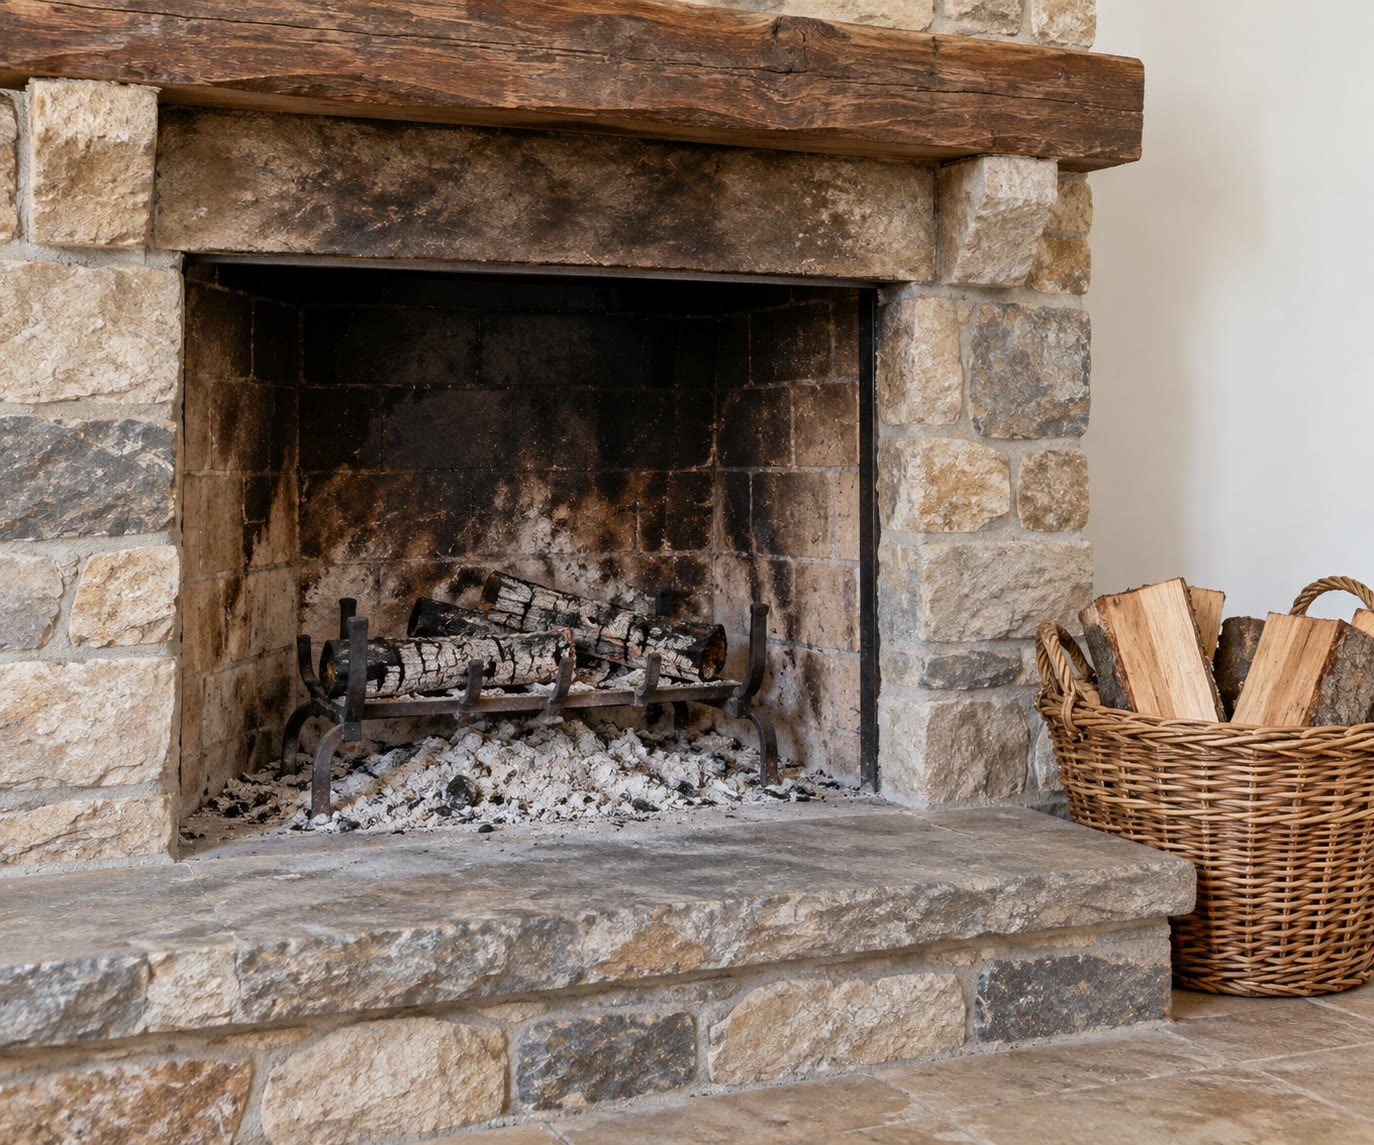
\includegraphics[width=0.5\linewidth]{images/book1/ai/g8-fireplace-ash.jpg}

{\small Uma lareira na manhã seguinte: um pouco de cinza é tudo o que
sobrou das toras.}
\end{omfigure}

\section{A massa se conserva}

\begin{inthelab}[Pesar uma reação num frasco fechado]
O professor põe um pouco de vinagre num erlenmeyer e bicarbonato de
sódio num balão de borracha encaixado no gargalo, depois coloca o
conjunto numa balança: \qty{212.4}{g}. O balão é levantado para que o
bicarbonato caia no vinagre: a \omterm{def:g6:pure-substances-and-mixtures:mixture}{mistura} borbulha e o balão incha com o
gás formado. A balança continua marcando \qty{212.4}{g}. A mesma reação
num frasco aberto, sem o balão, ``perde'' massa: o gás escapa para a
sala.
\end{inthelab}

\begin{omfigure}
\begin{tikzpicture}[font=\small, scale=1.15]
  % closed flask
  \pic[transform shape] at (0,0) {balance};
  \pic[transform shape] at (0,0.8) {erlenmeyer={0.25}{omWater!80}};
  \fill[red!55, draw=red!60!black] (0,4.05) ellipse (0.5 and 0.62);
  \fill[red!55] (-0.3,3.45) rectangle (0.3,3.6);
  \node[anchor=north, align=center] at (0,-0.1) {fechado: o gás fica\\ no balão};
  \node[anchor=west, font=\footnotesize] at (1.25,0.3) {\qty{212.4}{g}};
  % open flask
  \pic[transform shape] at (4,0) {balance};
  \pic[transform shape] at (4,0.8) {erlenmeyer={0.25}{omWater!80}};
  \foreach \y in {3.6,3.95,4.3} \draw[->, black!45, decorate,
    decoration={snake, amplitude=0.6pt, segment length=4pt}] (4,\y) -- (4,\y+0.3);
  \node[anchor=north, align=center] at (4,-0.1) {aberto: o gás escapa,\\ a leitura diminui};
  \node[anchor=west, font=\footnotesize] at (5.25,0.3) {\qty{211.9}{g}};
\end{tikzpicture}

{\small A mesma reação, pesada. No frasco fechado, a massa não muda; no
frasco aberto, o gás vai embora e a balança marca menos.}
\end{omfigure}

\begin{definition}[Conservação da massa]\label{def:g8:balanced-equations:conservation}
A \emph{conservação da massa}\index{conservacao da massa@conservação da massa} é a lei segundo
a qual, numa \omterm{def:g7:chemical-reactions:reaction}{reação química}, a massa total dos produtos formados é igual
à massa total dos \omterm{def:g7:chemical-reactions:reactant}{reagentes} consumidos. Nada se perde e nada se cria; a
matéria só muda de forma.
\end{definition}

\begin{example}[A tora, bem pesada]\label{ex:g8:balanced-equations:log}
Se fosse possível pesar a tora que \omterm{def:g4:what-a-fire-needs:burning}{queima} e o oxigênio que ela tirou do
\omterm{def:g4:air-a-mixture-of-gases:air}{ar} antes, e a cinza, o dióxido de carbono e o vapor de água depois, os
dois totais seriam iguais. A cinza é leve porque a maior parte dos
produtos são gases, que sobem pela chaminé.
\end{example}

\begin{history}[Lavoisier pesa tudo, de 1770 a 1789]
Antoine-Laurent Lavoisier tinha por regra pesar todas as substâncias
antes e depois de cada reação, em recipientes lacrados, para que nenhum
gás pudesse sair ou entrar. Ele mostrou que os metais ganham massa
quando enferrujam ou queimam, porque tiram alguma coisa do \omterm{def:g4:air-a-mixture-of-gases:air}{ar} --- o
oxigênio, que foi ele quem batizou --- e afirmou, em 1789, que numa
reação nada se cria e nada se perde. A esposa dele, Marie-Anne Paulze
Lavoisier, trabalhava ao seu lado, registrava os experimentos e
desenhou os aparelhos para o livro dele.
\end{history}

\begin{omfigure}
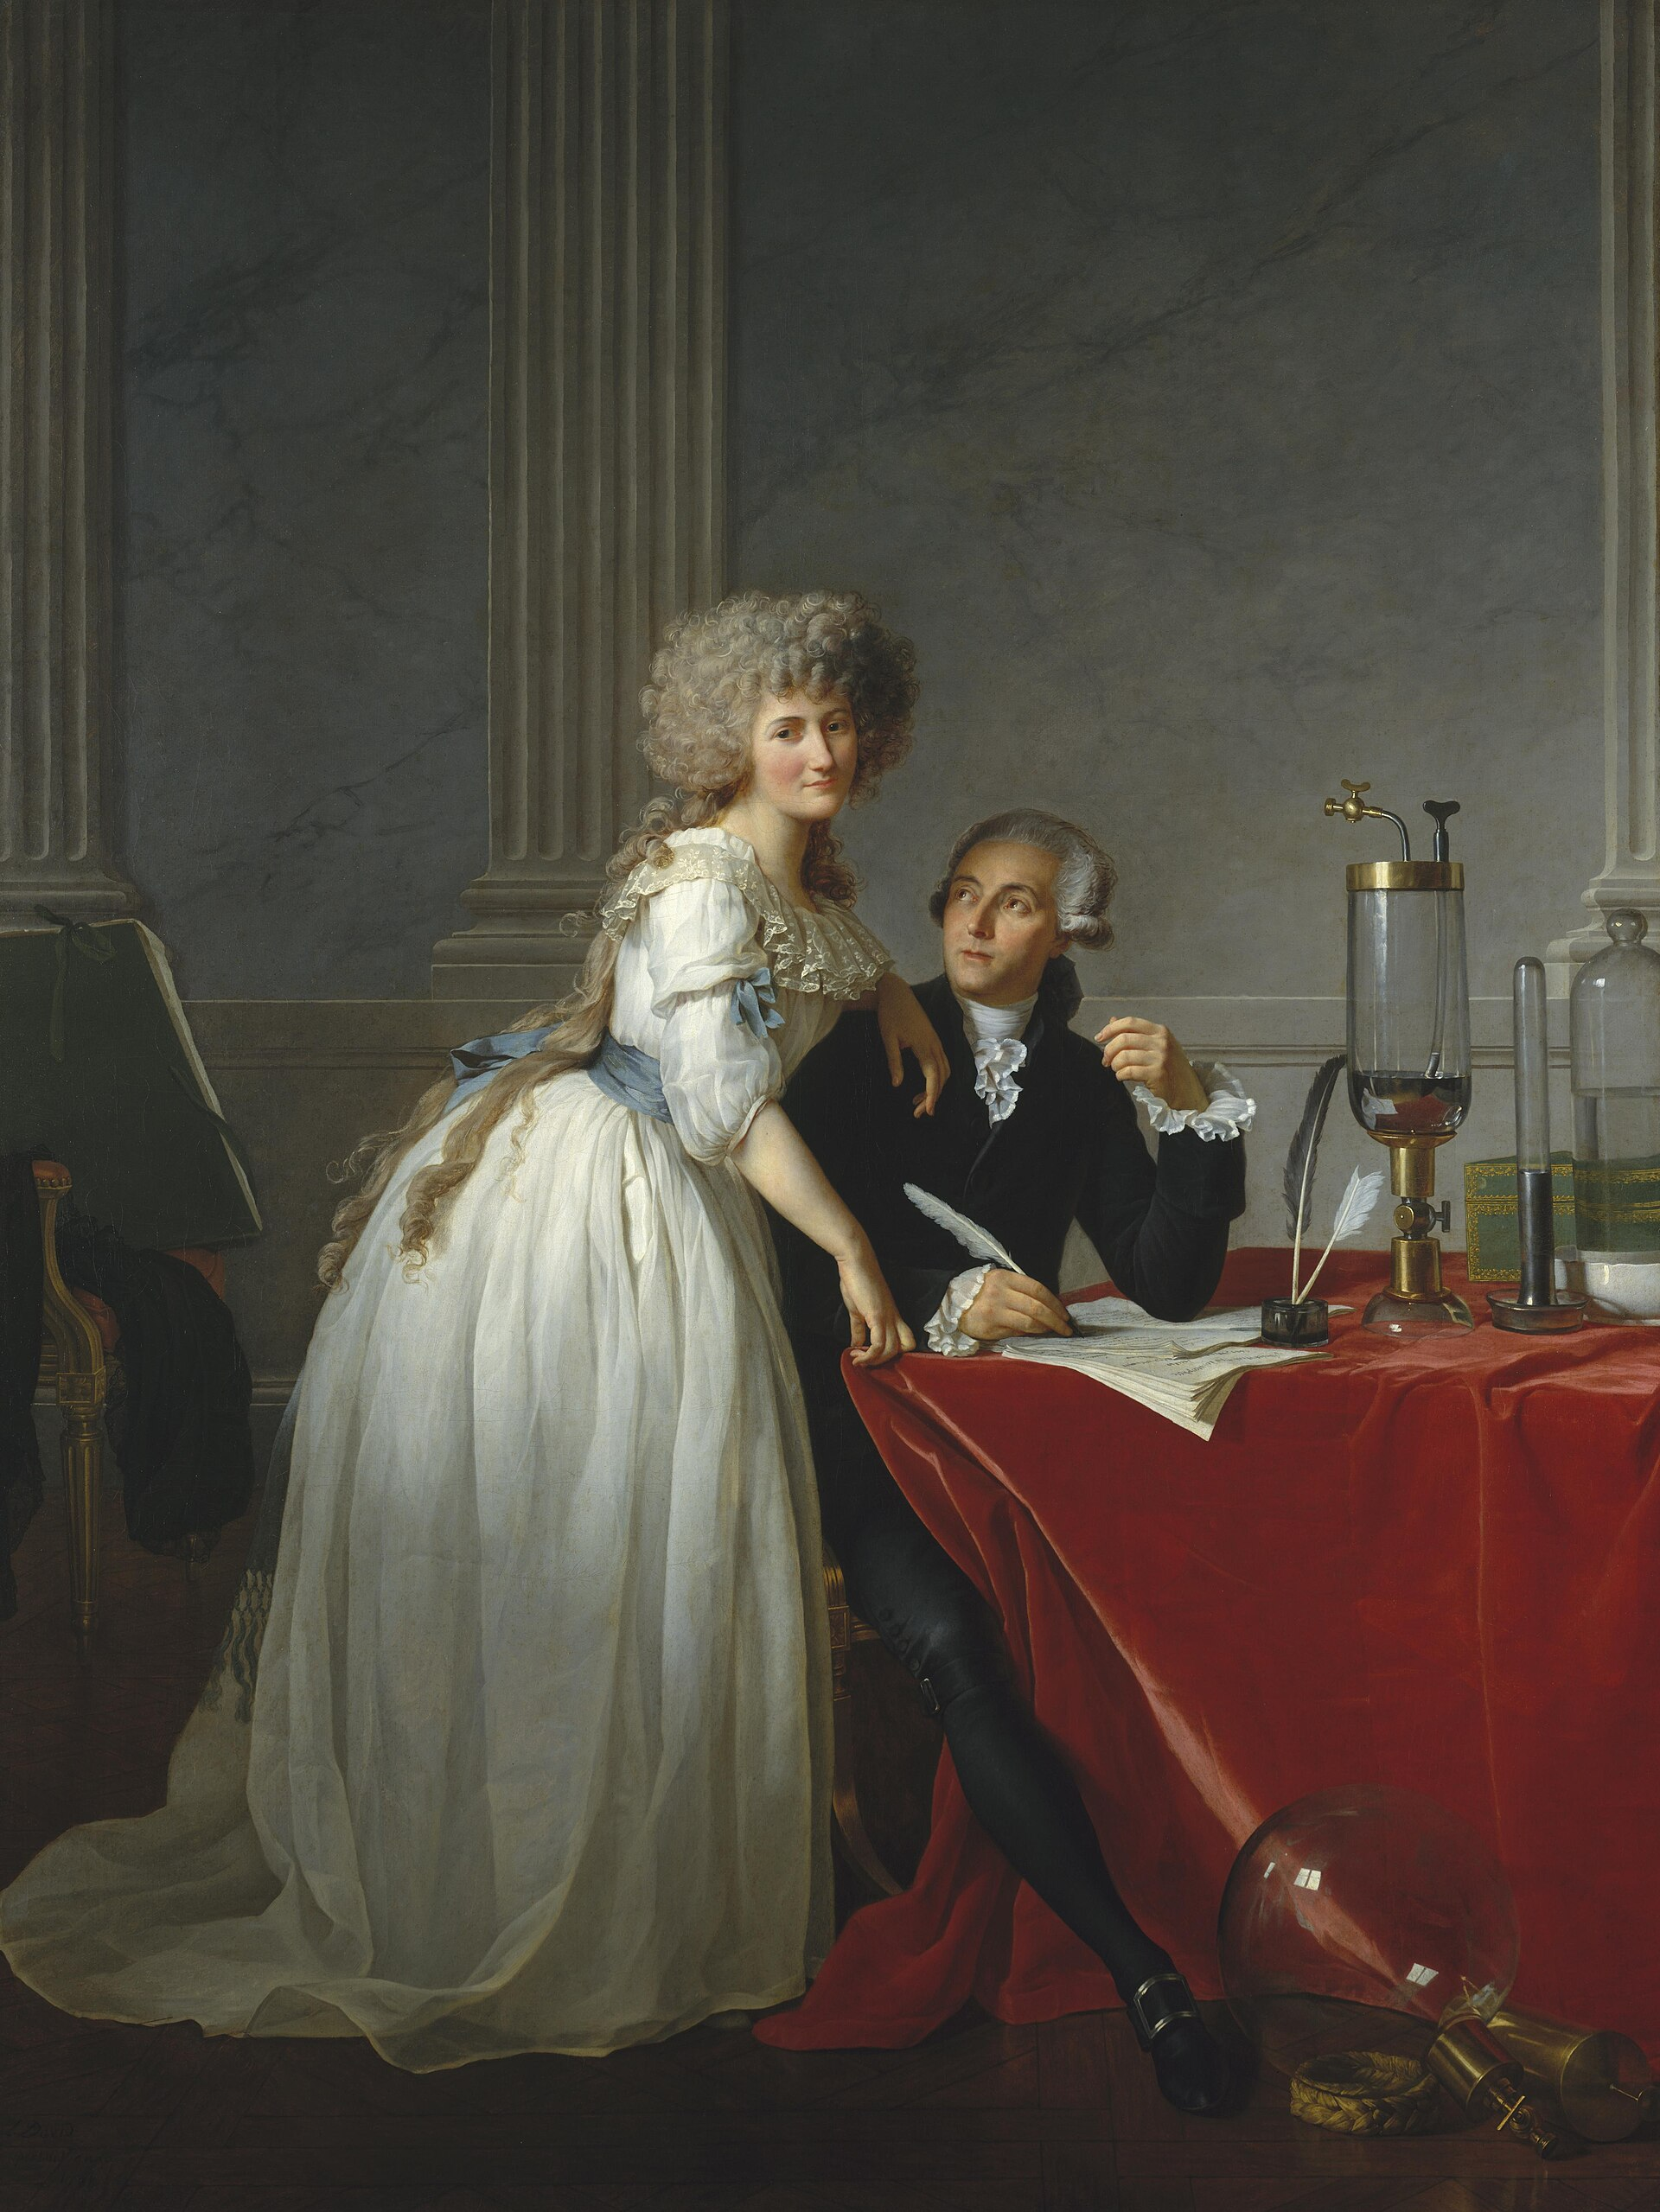
\includegraphics[width=0.3\linewidth]{images/book1/lavoisier.jpg}

{\small Antoine-Laurent Lavoisier e Marie-Anne Paulze Lavoisier, por
Jacques-Louis David, 1788.}
\end{omfigure}

\section{Por que a massa se conserva}

\begin{proposition}[Os átomos se conservam, logo a massa se conserva]\label{prop:g8:balanced-equations:why}
Numa reação, os \omterm{def:g7:atoms-and-molecules:atom}{átomos} só se rearranjam: cada \omterm{def:g7:atoms-and-molecules:atom}{átomo} dos \omterm{def:g7:chemical-reactions:reactant}{reagentes} é
encontrado de novo nos produtos. Cada \omterm{def:g7:atoms-and-molecules:atom}{átomo} conserva a sua própria
massa. Portanto, a massa total não pode mudar.
\end{proposition}

\begin{example}[O ferro que ganha massa]\label{ex:g8:balanced-equations:iron}
Palha de aço queimada numa balança, num prato aberto, fica mais pesada:
os \omterm{def:g7:atoms-and-molecules:atom}{átomos} de ferro se juntaram a \omterm{def:g7:atoms-and-molecules:atom}{átomos} de oxigênio tirados do \omterm{def:g4:air-a-mixture-of-gases:air}{ar}, e o
óxido de ferro formado pesa o ferro mais esse oxigênio. Queimada num
frasco lacrado cheio de \omterm{def:g4:air-a-mixture-of-gases:air}{ar}, em cima da balança, o conjunto não muda de
massa: o oxigênio já estava dentro do frasco.
\end{example}

\section{A equação química}

\begin{definition}[Equação química]\label{def:g8:balanced-equations:equation}
Uma \emph{equação química}\index{equacao quimica@equação química} escreve uma reação com
fórmulas: as fórmulas dos \omterm{def:g7:chemical-reactions:reactant}{reagentes} à esquerda, ligadas por $+$, uma
seta, e as fórmulas dos produtos à direita. Cada fórmula pode ter um
número na frente. A equação é uma
\emph{equação balanceada}\index{equacao balanceada@equação balanceada} quando cada tipo de
\omterm{def:g7:atoms-and-molecules:atom}{átomo} aparece o mesmo número de vezes dos dois lados.
\end{definition}

\begin{definition}[Coeficiente estequiométrico]\label{def:g8:balanced-equations:coefficient}
O número escrito na frente de uma fórmula numa equação é o seu
\emph{coeficiente estequiométrico}\index{coeficiente estequiometrico@coeficiente estequiométrico}:
ele conta as \omterm{def:g7:atoms-and-molecules:molecule}{moléculas} (ou outras partículas) dessa espécie que
participam. O coeficiente 1 não é escrito.
\end{definition}

\begin{notation}[Indicação do estado físico]\label{not:g8:balanced-equations:states}
Uma letra entre parênteses depois de uma fórmula pode indicar o estado
físico: (s) sólido, (l) líquido, (g) gasoso. Assim, \ce{H2O(l)} é a água
líquida e \ce{H2O(g)}, o vapor de água.
\end{notation}

\begin{example}[Ler uma equação]\label{ex:g8:balanced-equations:read}
\[
  \ce{CH4(g) + 2O2(g) -> CO2(g) + 2H2O(l)}
\]
se lê: uma \omterm{def:g7:atoms-and-molecules:molecule}{molécula} de metano e duas \omterm{def:g7:atoms-and-molecules:molecule}{moléculas} de oxigênio reagem e dão
uma \omterm{def:g7:atoms-and-molecules:molecule}{molécula} de dióxido de carbono e duas \omterm{def:g7:atoms-and-molecules:molecule}{moléculas} de água. À esquerda:
1 C, 4 H, 4 O. À direita: 1 C, 4 H, $2 + 2 = 4$ O. A equação está
balanceada.
\end{example}

\begin{omfigure}
\begin{tikzpicture}[font=\small]
  \begin{scope}[every node/.style={font=\Large, inner sep=2pt}]
    \node (a) at (0,0) {\ce{CH4}};
    \node (p1) at (0.95,0) {$+$};
    \node (b) at (1.9,0) {\ce{2O2}};
    \node (arr) at (3.35,0) {$\longrightarrow$};
    \node (c) at (4.8,0) {\ce{CO2}};
    \node (p2) at (5.75,0) {$+$};
    \node (d) at (6.8,0) {\ce{2H2O}};
  \end{scope}
  \draw[thick, omDef] ([yshift=-2pt]a.south west) -- ++(0,-0.15) -| ([yshift=-2pt]b.south east);
  \node[below=8pt, text=black] at ($(a.south)!0.5!(b.south)$) {reagentes};
  \draw[thick, omProp] ([yshift=-2pt]c.south west) -- ++(0,-0.15) -| ([yshift=-2pt]d.south east);
  \node[below=8pt, text=black] at ($(c.south)!0.5!(d.south)$) {produtos};
  \node[above=6pt of arr, font=\small] {``reagem e dão''};
  \node[anchor=north west, align=left, draw=black!35, rounded corners=2pt,
    font=\small, inner sep=4pt] at (-0.3,-1.25)
    {Em \ce{2O2}: o 2 grande na frente é o \textbf{coeficiente} (duas moléculas);\\
     o 2 pequeno abaixo da linha é o \textbf{índice} (dois átomos em cada molécula).};
\end{tikzpicture}

{\small As partes de uma \omterm{def:g8:balanced-equations:equation}{equação química}.}
\end{omfigure}

\section{Balancear uma equação}

\begin{method}[Balancear uma equação]\label{met:g8:balanced-equations:balance}
\begin{enumerate}
  \item Escreva as fórmulas corretas dos \omterm{def:g7:chemical-reactions:reactant}{reagentes} e dos produtos. Nunca
        mude uma fórmula depois: transformar \ce{H2O} em \ce{H2O2}
        descreveria outra substância.
  \item Conte os \omterm{def:g7:atoms-and-molecules:atom}{átomos} de cada tipo de cada lado.
  \item Balanceie um tipo de \omterm{def:g7:atoms-and-molecules:atom}{átomo} de cada vez com coeficientes,
        começando pelos \omterm{def:g7:atoms-and-molecules:atom}{átomos} que aparecem numa só fórmula de cada lado;
        deixe o hidrogênio e o oxigênio para o fim.
  \item Conte de novo; repita até que todos os tipos de \omterm{def:g7:atoms-and-molecules:atom}{átomo} estejam
        balanceados.
  \item Use os menores números inteiros.
\end{enumerate}
\end{method}

\begin{example}[Hidrogênio e oxigênio]\label{ex:g8:balanced-equations:water}
Não balanceada: \ce{H2 + O2 -> H2O} % ce-unbalanced-ok (the skeleton)
tem 2 O à esquerda e 1 à direita. Ponha 2 na frente de \ce{H2O}: agora
há 4 H à direita, então 2 na frente de \ce{H2}:
\[
  \ce{2H2 + O2 -> 2H2O}.
\]
Verificação: 4 H e 2 O de cada lado.
\end{example}

\begin{example}[O ferro queimando no oxigênio]\label{ex:g8:balanced-equations:iron-oxide}
O ferro e o oxigênio dão o óxido de ferro \ce{Fe2O3}. Oxigênio: 2 à
esquerda, 3 à direita; o menor número comum é 6, então 3 \ce{O2} e 2
\ce{Fe2O3}. Ficam 4 Fe à direita, então 4 Fe à esquerda:
\[
  \ce{4Fe + 3O2 -> 2Fe2O3}.
\]
\end{example}

\begin{omfigure}
\begin{tikzpicture}[font=\small]
  % 2 H2
  \foreach \y in {0.45,-0.45} {
    \node[aH] (a) at (0,\y) {}; \node[aH] (b) at (0.45,\y) {};
    \begin{scope}[on background layer]\draw[bond] (a.center) -- (b.center);\end{scope}}
  \node at (1.05,0) {$+$};
  \node[aO] (a) at (1.6,0) {}; \node[aO] (b) at (2.25,0) {};
  \begin{scope}[on background layer]
    \draw[bond, line width=1.1pt] ([yshift=1.6pt]a.center) -- ([yshift=1.6pt]b.center);
    \draw[bond, line width=1.1pt] ([yshift=-1.6pt]a.center) -- ([yshift=-1.6pt]b.center);
  \end{scope}
  \draw[->, thick, omProp] (2.9,0) -- (3.9,0);
  \foreach \y in {0.5,-0.5} {
    \node[aO] (o) at (4.9,\y+0.12) {};
    \node[aH] (p) at (4.35,\y-0.28) {}; \node[aH] (q) at (5.45,\y-0.28) {};
    \begin{scope}[on background layer]
      \draw[bond] (o.center) -- (p.center); \draw[bond] (o.center) -- (q.center);
    \end{scope}}
  \node[align=center, font=\footnotesize] at (1.1,-1.35) {4 H, 2 O};
  \node[align=center, font=\footnotesize] at (4.9,-1.35) {4 H, 2 O};
  \node[font=\small] at (2.7,-2.0) {\ce{2H2 + O2 -> 2H2O}};
\end{tikzpicture}

{\small A \omterm{def:g8:balanced-equations:equation}{equação balanceada} da \omterm{def:g4:what-a-fire-needs:burning}{queima} do hidrogênio, desenhada com
modelos: duas \omterm{def:g7:atoms-and-molecules:molecule}{moléculas} de hidrogênio e uma \omterm{def:g7:atoms-and-molecules:molecule}{molécula} de oxigênio dão
duas \omterm{def:g7:atoms-and-molecules:molecule}{moléculas} de água.}
\end{omfigure}

\section{Ler uma equação em moléculas}


\begin{proposition}[O que uma equação balanceada diz]\label{prop:g8:balanced-equations:molecules}
Os coeficientes de uma \omterm{def:g8:balanced-equations:equation}{equação balanceada} dão as proporções em que as
partículas reagem e são formadas. Se a equação diz
\ce{2H2 + O2 -> 2H2O}, então 200 \omterm{def:g7:atoms-and-molecules:molecule}{moléculas} de hidrogênio reagem com 100
\omterm{def:g7:atoms-and-molecules:molecule}{moléculas} de oxigênio e dão 200 \omterm{def:g7:atoms-and-molecules:molecule}{moléculas} de água; um milhão de
\omterm{def:g7:atoms-and-molecules:molecule}{moléculas} de oxigênio precisam de dois milhões de \omterm{def:g7:atoms-and-molecules:molecule}{moléculas} de
hidrogênio.
\end{proposition}

\begin{example}[O propano de um fogareiro de camping]\label{ex:g8:balanced-equations:propane}
O propano, \ce{C3H8}, \omterm{def:g4:what-a-fire-needs:burning}{queima} no oxigênio e dá dióxido de carbono e água.
Primeiro o carbono: 3 C, então 3 \ce{CO2}. Hidrogênio: 8 H, então 4
\ce{H2O}. Oxigênio à direita: $3 \times 2 + 4 = 10$ O, então 5 \ce{O2}:
\[
  \ce{C3H8 + 5O2 -> 3CO2 + 4H2O}.
\]
Cada \omterm{def:g7:atoms-and-molecules:molecule}{molécula} de propano precisa de cinco \omterm{def:g7:atoms-and-molecules:molecule}{moléculas} de oxigênio.
\end{example}

\section{Exercícios}

\begin{exercise}[$\star$]\label{exo:g8:balanced-equations:1}
Enuncie a lei de \omterm{def:g8:balanced-equations:conservation}{conservação da massa}.
\end{exercise}

\begin{exercise}[$\star$]\label{exo:g8:balanced-equations:2}
Em \ce{3CO2}, qual é o \omterm{def:g8:balanced-equations:coefficient}{coeficiente estequiométrico}? Quantos \omterm{def:g7:atoms-and-molecules:atom}{átomos} de
carbono e quantos \omterm{def:g7:atoms-and-molecules:atom}{átomos} de oxigênio ele representa?
\end{exercise}

\begin{exercise}[$\star$]\label{exo:g8:balanced-equations:3}
A equação \ce{C + O2 -> CO2} está balanceada? Conte os \omterm{def:g7:atoms-and-molecules:atom}{átomos} para
verificar.
\end{exercise}

\begin{exercise}[$\star$]\label{exo:g8:balanced-equations:4}
Balanceie \ce{Mg + O2 -> MgO}. % ce-unbalanced-ok (to balance)
\end{exercise}

\begin{exercise}[$\star\star$]\label{exo:g8:balanced-equations:5}
Balanceie \ce{N2 + H2 -> NH3}, a reação que produz a amônia. % ce-unbalanced-ok (to balance)
\end{exercise}

\begin{exercise}[$\star\star$]\label{exo:g8:balanced-equations:6}
\qty{12}{g} de carbono queimam completamente e formam \qty{44}{g} de
dióxido de carbono. Que massa de oxigênio foi consumida?
\end{exercise}

\begin{exercise}[$\star\star$]\label{exo:g8:balanced-equations:7}
Olhe a figura dos dois frascos nas balanças. Por que a leitura do frasco
aberto diminui? Massa foi destruída?
\end{exercise}

\begin{exercise}[$\star\star$]\label{exo:g8:balanced-equations:8}
Balanceie \ce{CH4 + O2 -> CO2 + H2O} passo a passo, dizendo que \omterm{def:g7:atoms-and-molecules:atom}{átomo} % ce-unbalanced-ok (to balance)
você balanceia em cada passo.
\end{exercise}

\begin{exercise}[$\star\star$]\label{exo:g8:balanced-equations:9}
Um aluno balanceia \ce{H2 + O2 -> H2O} escrevendo \ce{H2 + O2 -> H2O2}. % ce-unbalanced-ok (the student's start)
Por que isso está errado?
\end{exercise}

\begin{exercise}[$\star\star$]\label{exo:g8:balanced-equations:10}
Com \ce{C3H8 + 5O2 -> 3CO2 + 4H2O}, quantas \omterm{def:g7:atoms-and-molecules:molecule}{moléculas} de oxigênio são
necessárias para queimar 20 \omterm{def:g7:atoms-and-molecules:molecule}{moléculas} de propano? Quantas \omterm{def:g7:atoms-and-molecules:molecule}{moléculas} de
água são formadas?
\end{exercise}

\begin{exercise}[$\star\star\star$]\label{exo:g8:balanced-equations:11}
Balanceie \ce{C2H6 + O2 -> CO2 + H2O}, a \omterm{def:g4:what-a-fire-needs:burning}{queima} do etano. (Dica: tente % ce-unbalanced-ok (to balance)
dobrar o etano.)
\end{exercise}

\begin{exercise}[$\star\star\star$]\label{exo:g8:balanced-equations:12}
Uma vela de \qty{20.0}{g} \omterm{def:g4:what-a-fire-needs:burning}{queima} numa caixa de vidro lacrada cheia de
\omterm{def:g4:air-a-mixture-of-gases:air}{ar}, que está sobre uma balança que marca \qty{850.0}{g} ao todo. Quando a
chama se apaga, a vela pesa \qty{19.6}{g}. Quanto a balança marca?
Explique.
\end{exercise}

\section{Problema: palha de aço num frasco lacrado}

\begin{problem}[{Problema de fim de semana --- um ferro que queima, uma
balança que não se mexe e o oxigênio tirado do ar}]
\label{pb:g8:balanced-equations:1}
Num laboratório, um professor \omterm{def:g4:what-a-fire-needs:burning}{queima} palha de aço, que é ferro quase
puro, de dois jeitos. Primeiro, um chumaço é queimado num prato aberto
sobre uma balança: a leitura aumenta. Depois, um chumaço de
\qty{0.28}{g} é queimado, aceso por uma faísca elétrica, dentro de um
frasco fechado cheio de \omterm{def:g4:air-a-mixture-of-gases:air}{ar}, colocado sobre a balança: a leitura não
muda. O frasco contém cerca de \qty{0.5}{g} de oxigênio. O ferro que
\omterm{def:g4:what-a-fire-needs:burning}{queima} no oxigênio forma o óxido de ferro \ce{Fe2O3}; com menos oxigênio,
ele também pode formar \ce{Fe3O4}.

\medskip
\noindent\textbf{Parte I --- Duas pesagens.}
\begin{enumerate}
  \item No prato aberto, a massa aumenta. De onde vem a massa a mais?
  \item No frasco fechado, a massa não muda. Explique.
  \item Enuncie a lei ilustrada por essas duas pesagens.
\end{enumerate}

\medskip
\noindent\textbf{Parte II --- Duas equações.}
\begin{enumerate}[resume]
  \item Balanceie a equação \ce{Fe + O2 -> Fe2O3}. % ce-unbalanced-ok (to balance)
  \item Balanceie a equação \ce{Fe + O2 -> Fe3O4}. % ce-unbalanced-ok (to balance)
  \item Verifique a primeira equação contando os \omterm{def:g7:atoms-and-molecules:atom}{átomos} de cada tipo de
        cada lado.
  \item Segundo a primeira equação, quantas \omterm{def:g7:atoms-and-molecules:molecule}{moléculas} de oxigênio reagem
        com 400 \omterm{def:g7:atoms-and-molecules:atom}{átomos} de ferro?
\end{enumerate}

\medskip
\noindent\textbf{Parte III --- Massas.}
No \ce{Fe2O3}, cada \qty{7}{g} de ferro estão combinados com \qty{3}{g}
de oxigênio. O chumaço de \qty{0.28}{g} \omterm{def:g4:what-a-fire-needs:burning}{queima} completamente e vira
\ce{Fe2O3}.
\begin{enumerate}[resume]
  \item Que massa de oxigênio se combina com \qty{0.28}{g} de ferro?
  \item Qual é a massa de óxido de ferro formada?
  \item Havia oxigênio suficiente no frasco? Explique.
  \item O frasco é aberto depois de esfriar, e o \omterm{def:g4:air-a-mixture-of-gases:air}{ar} entra com força.
        Explique por quê, e diga como a leitura da balança muda então.
  \item Calcule a massa de oxigênio tirada do \omterm{def:g4:air-a-mixture-of-gases:air}{ar} do frasco pela palha de
        aço que queimou.
\end{enumerate}
\end{problem}
